%//==============================--@--==============================//%
\clearpage
\subsection{2.2 Modelação de Ângulo (PM e FM)}
\label{subsubsec:PM-FM}

Seja $\theta_i(t)$ o ângulo da portadora sinusoidal modulada que transporta o sinal mensagem. Exprime-se a resultante onde modulada como:
$$
    \boxed{ s(t) = A_c \cos\left[\theta_i(t)\right] }
    \quad \implies \quad
    f_i(t) = \frac{1}{2\pi} \frac{d \theta_i(t)}{dt}
$$

\begin{enumerate}
    \item[$\pmb{1.}$] \textit{Phase modulation} (PM): ``form of angle modulation in which the instantaneous angle $\theta_i(t)$ is varied linearly with the message signal $m(t)$''
    $$
        \pmb{\rightarrow} \theta_i(t) = 2\pi f_c t + k_p m(t)
    $$
    $$
        \therefore x_{\text{PM}}(t) = A_c \cos\left[ 2\pi f_c t + k_p m(t) \right]
    $$

    \item[$\pmb{2.}$] \textit{Frequency modulation} (FM): ``form of angle modulation in which the instanta- neous frequency $f_i(t)$ is varied linearly with the message signal $m(t)$''
    $$
        \pmb{\rightarrow} f_i(t) = f_c + f_\Delta\, m(t)
    $$
    $$
        \therefore x_{\text{FM}}(t) = A_c \cos\left[ 2\pi f_c t + 2\pi f_\Delta \int_{0}^{t} m(\tau) \, d\tau \right]
    $$
\end{enumerate}

\noindent em que $k_f$ representa o fator de \textit{phase-sensivity}, e $f_\Delta$ a \textit{frequency deviation}.
%//==============================--@--==============================//%
\subsubsection[2.2.1 Relação entre PM e FM]{$\rightarrow$ Relação entre PM e FM}
\label{subsubsec:PM-FM-relation}

Tendo em conta as definições acima, é natural verificar que um modulador de fase é realizável através de um modulador de frequência, e vice-versa.
%Adoro-te
\begin{figure}[H]
    \centering
    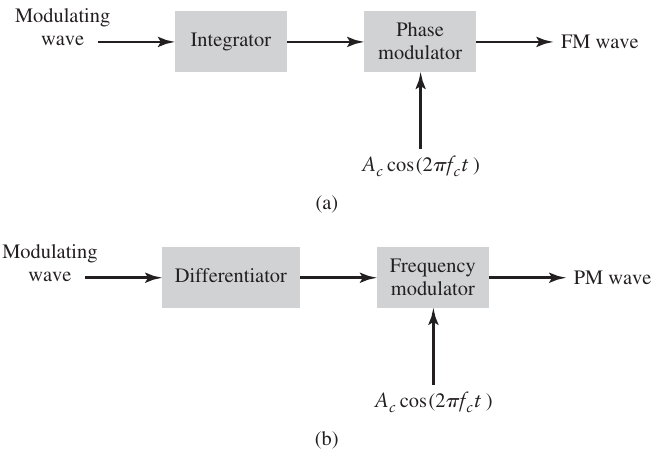
\includegraphics[width = 0.5\linewidth]{img/analog/FM/PM-FM-relation.png}
    \caption{``Illustration of the relationship between $[$FM$]$ and $[$PM$]$. (a) Scheme for generating an FM wave by using a phase modulator. (b) Scheme for generating a PM wave by using a frequency modulator.''\cite{Haykin2007}}
    \label{fig:PM-FM-relation}
\end{figure}

%//==============================--@--==============================//%
\subsubsection[2.2.2 Largura de banda FM (Carson's rule)]{$\rightarrow$ Largura de banda FM (Carson's rule)}
\label{subsubsec:FM}

\begin{theo}[\underline{Carson's rule} \cite{Haykin2007}]{def:carsons-rule}\label{def:carsons-rule}
$$
    B_T = 2(\beta + 1)W,\qquad \beta = \frac{f_\Delta\, \left[\text{max}\{m(t)\} - \text{min}\{m(t)\}\right]/2}{W}
$$
em que $\beta$ é o índice de modulação.
\end{theo}

\noindent ``The Carson’s rule shows that, for $\beta > 1$ (wideband FM), the bandwidth of the FM signals is much larger than that of the AM signals, for a given value of $W$.''\cite{Nunes2015}

\newpage

\iffalse
\noindent $\pmb{\rightarrow}$ \textbf{Nota:} ``The Carson’s rule provides sometimes a too small bandwidth estimate. A more approximated expression, for $\beta > 2$, would be $B_T = 2(\beta + 2)W$''\cite{Nunes2015}.
\fi

%//==============================--@--==============================//%
\paragraph[2.2.2.1 FM de banda estreita]{$\pmb{\star}$ FM de banda estreita (\textit{narrow-band})}\mbox{}\\
\noindent Supondo que $f_\Delta$ é tal que  
$$
    \left| 2\pi f_\Delta \int_{0}^{t} m(\tau)\, d\tau \right| \ll 1
$$
então
\begin{align*}
    x_{\text{FM}}(t) &= A_c \cos(2\pi f_c t) \cos( 2\pi f_\Delta \int_{0}^{t} m(\tau)\, d\tau ) - A_c \sin(2\pi f_c t) \sin( 2\pi f_\Delta \int_{0}^{t} m(\tau)\, d\tau ) \\
                     &\approx A_c \cos(2\pi f_c t) - A_c \sin(2\pi f_c t) \cdot \left( 2\pi f_\Delta \int_{0}^{t} m(\tau)\, d\tau \right)
\end{align*}
Isto indica que o sinal de banda estreita se aproxima de um sinal AM. Deste modo, a largura de banda será
$$
    B_T \approx 2B
$$
em que $B$ é a largura de banda do sinal fonte $m(t)$.

%//==============================--@--==============================//%
\paragraph[2.2.2.2 FM de banda larga]{$\pmb{\star}$ FM de banda larga (\textit{wide-band})}\mbox{}\\
Neste caso, temos que $f_\Delta \gg B$. A análise do sinal FM de banda larga é de natureza não trivial, pelo que se apresenta o ponto fulcral.
\\[6pt]
\noindent \textbf{Aproximação quasi-estacionária:} Caso $f_c \gg f_\Delta \gg B$, o espectro de potência do sinal FM é (aproximadamente) dado por:
$$
    S_x(f) = \frac{A^2}{4f_\Delta}\left[ f_x\left( -\frac{f+f_c}{f_\Delta} \right) + f_x\left( \frac{f-f_c}{f_\Delta} \right) \right]
$$
em que $f_x$ é a função de densidade de probabilidade.
\\[6pt]
\noindent Nestes moldes,
$$
     B_T \approx f_\Delta \cdot \left[ \text{max}\{m(t)\} - \text{min}\{m(t)\} \right]
$$
%//==============================--@--==============================//%
\subsubsection[2.2.3 Potência de transmissão de uma onda modulada em ângulo]{$\rightarrow$ Potência de transmissão de uma onda modulada em ângulo}
\label{subsubsec:FM-power}

Verifica-se que a amplitude de ondas PM e FM, $A_c$, se mantém constante ao longo do tempo, indepentemente do valor de $k_p$ ou de $f_\Delta$. Consequentemente, a potência média transmitida é uma contante dada por:
$$
    P_T = \frac{1}{2}A^2_c
$$
(é assumido que a resistência da carga é $1$ ohm).
%//==============================--@--==============================//%
\subsubsection[2.2.4 Discriminador de frequência (desmodulação de uma onda FM)]{$\rightarrow$ Discriminador de frequência (desmodulação de uma onda FM)}
\label{subsubsec:FM-discriminador}

\begin{figure}[H]
    \centering
    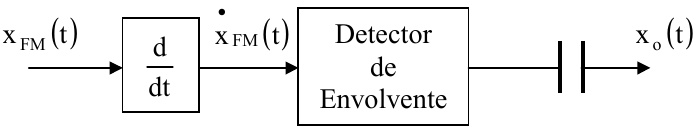
\includegraphics[width = 0.5\linewidth]{img/analog/FM/discriminadorFM.png}
    \caption{Discriminador de frequência\cite{Victor2010}.}
    \label{fig:FM-discriminador}
\end{figure}

$$
    \dot{x}_{FM}(t) = -2\pi A_c \left( f_c + f_\Delta m(t) \right) \sin(2\pi f_c t + 2\pi f_\Delta \int_{0}^{t} m(\tau)\, d\tau)
$$
 A saída do diferenciador não é mais do que uma portadora sinusoidal cuja envolvente vale $2\pi A_c (f_c + f_\Delta m(t))$, deste modo:
$$
    \because f_c \gg f_\Delta \implies x_0(t)\: \propto\: m(t)
$$
%//==============================--@--==============================//%